\documentclass[a4paper,11pt]{article}

\sloppy

\usepackage[T1]{fontenc}
\usepackage[utf8x]{inputenc}
\usepackage[pdftex]{graphics}
\usepackage[ngerman]{babel}
\usepackage{graphicx} 
\usepackage{tabularx}
\usepackage{amsmath,amssymb,amstext}
\usepackage{bibtopic}
\usepackage{float}
\usepackage{hyperref}
\usepackage{multirow}
\usepackage{listings}
\usepackage{a4wide}
\usepackage{verbatim}
%\usepackage{geometry}

\renewcommand{\lstlistingname}{\normalsize Quellcode}
\renewcommand{\lstlistlistingname}{Verzeichnis der Quellcodes}
\let\stdsection\section
%\renewcommand{\section}{\newpage\stdsection}

%\pagestyle{plain}
\bibliographystyle{alpha}

\newcommand{\cmacro}[1]{\mbox{\textsc{#1}}}
\newcommand{\wochendatumnonew}[2]{\subsection[#2]{#2\\\textmd{#1}}}
\newcommand{\wochendatum}[2]{\newpage \wochendatumnonew{#1}{#2}}

\title{
	\textbf{Exposé zur Bachelor-Thesis ``Integration von HomeMatic-Komponenten in eine AAL-Plattform''}
}
\author{
	\textit{Mierswa, Daniel} \\
	Matrikelnummer: 561378 \\
	daniel.mierswa@student.hs-rm.de \\
}

\newcommand{\abstractspace}{\vspace*{0.3cm}\rule{0.75\textwidth}{0.4pt}\vspace*{0.3cm}}

\date{29. September 2013}

\begin{document}
\maketitle

\section{Problemfeld}
Die Abschlussarbeit soll zeigen, wie Hausautomationsgeräte, aus dem HomeMatic-System in die
AAL-Plattform WieDAS integriert werden können.
Ein solches System besteht aus Sensoren und Aktoren.
HomeMatic verwendet ein proprietäres Funkprotokoll.
Ein Zugriff auf die Geräte ist über eine vom Hersteller spezifizierte XML-Schnittstelle möglich.
In der Arbeit soll eine Gateway-Komponente (Connector) entwickelt werden, die diese XML-Schnittstelle
verwendet, um Geräte in die WieDAS-Dienstplattform einzubinden.

\section{Zielsetzung}
Das grundlegende Ziel ist es, dass die WieDAS-Dienstplattform in der Lage ist, mit HomeMatic-Geräten zu
kommunizieren und gewünschte Daten aus dem sogenannten Cache abzurufen bzw. in diesen einzupflegen.
Die Basisplattform von WieDAS besteht aus mehreren Schichten (Sensorik, Hardware, Cache und Logik) und
wurde im Rahmen eines Forschungsprojekts entwickelt.
Schlussendlich soll ein Cache-Connector die HomeMatic-Geräte an den WieDAS-Cache anbinden.
Das WieDAS-Datenmodell, sowie die HomeMatic-Geräte müssen vorher hinreichend analysiert werden, um mögliche
Abbildungen zu entwickeln.
Weiterhin müssen die verwendeten Schnittstellen vom WieDAS-Cache und HomeMatic betrachtet werden.
Eine modulare  Implementierung ist vorgesehen, so dass zukünftig erstellte Geräte in der Lage sind einfach
an die WieDAS-Dienstplattform angebunden zu werden.
Es ist denkbar, dass der Connector neue Geräte über dynamisch geladene Bibliotheken einbindet.

\section{Methodik}
Zuerst werden grundlegende Kenntnisse über die WieDAS-Platform und die HomeMatic Schnittstelle gewonnen.
Dabei ist es wichtig, die große Menge von Informationen entsprechend zu filtern und nur relevante Dokumentation
zu lesen.
Für die Thesis ist es z.B. nicht von großer Bedeutung, wie die WieDAS-Dienstplattform und die HomeMatic-Schnittstelle
auf den Geräten implementiert ist.
Währenddessen wird eine Gliederung für die Abschlussarbeit festgelegt und in einem TeX-Dokument hinterlegt.
Die Abschlussarbeit und die dazugehörige Daten werden in ``svn repositories'' des Labors für Verteilte Systeme
gepflegt.
Die Arbeiten werden so durchgeführt, dass Arbeitsschritte stets dokumentiert werden.
Da bereits eine Vielfalt von HomeMatic-Geräten existiert, wird in der Hochschule recherchiert, wie diese
in der Praxis funktionieren und wie die XML-Schnittstelle implementiert ist.
Aufgrund der gesammelten Informationen soll anschließend festgelegt werden, wie der Cache-Connector zu entwickeln ist.
Die Implementierung soll objektorientiert geschehen.
Es wird ein sehr abstraktes Basisobjekt entwickelt, welches von den spezifische Geräten benutzt wird.
Die Geräte können in einer IDL modelliert werden.
Die Datenbeschreibung kann von Geräten, die im WieDAS-Projekt unterstützt sind, entnommen werden.
Um die Integration zu testen, werden HomeMatic-Aktoren über WieDAS gesteuert und gleichzeitig wird geprüft, ob die
HomeMatic-Sensoren den WieDAS-Cache erreichen, z.B. über das Aufleuchten von LEDs oder anderen Statusanzeigen.

\section{Erwartete Ergebnisse}
Der Cache der WieDAS-Dienstplattform soll in der Lage sein, HomeMatic-Geräte zu integrieren.
Dazu wird auf einem Gerät der Cache-Connector implementiert, welcher über das Netzwerk mit dem AAL-Cache und
der HomeMatic-Zentrale kommuniziert.
Die Integration geschieht über Abbildungen der Datenmodelle von HomeMatic und WieDAS und der Implementierung
der XML-RPC-Aufrufe und Abarbeitungen.
Es sind Abbildungen für die WieDAS-Projekt unterstützen Geräte vorgesehen.
Optional soll der Connector in der Lage sein, neue Geräte über dynamisch-ladbare Bibliotheken (z.B. mit Einstecken
eines USB-Sticks) anzubinden.

\section{Zeitplan}
Der erste Schritt ist die Recherche über den Cache und die XML-RPC-Schnittstelle, sowie der Beginn der Gliederung
der Thesis.
Nach den ersten 2 Wochen sollte eine Anforderungsanalyse bereitstellen, die mit den Betreuern diskutiert werden kann.
Mit dieser kann dann die Designphase gestartet werden, in welcher es noch passieren kann, dass Verbesserungsvorschläge
aus der Analyse mit einfließen und Korrekturen darin vorgenommen werden müssen.
Nach einem Monat sollte die Designphase zunächst abgeschlossen sein und mit den Betreuern besprochen werden.
Da zu diesem Zeitpunkt 2 wesentliche Aspekte der Thesis zumindest zur Vorlage bereit sind, sollte auch die Gliederung
bis dahin spätestens fertiggestellt sein.
Nach 5 Wochen sollte die Implementierungsphase beginnen.
Nach 6 Wochen muss die Designphase und Anforderungsanalyse soweit fertig sein, so dass die Implementierungsphase
nicht mehr durch Designveränderungen beeinträchtigt wird.
Zu diesem Zeitpunkt sollte auch der strukturierte Teil der beiden Phasen im Dokument niedergeschrieben worden sein und
nicht weiter bearbeitet werden.
Die Implementierungsphase sollte 3-5 Wochen dauern, so dass am Ende der Abschlussarbeit 2 Wochen Zeit bleiben Fazite
zu ziehen und Verbesserungsvorschläge einzubauen.

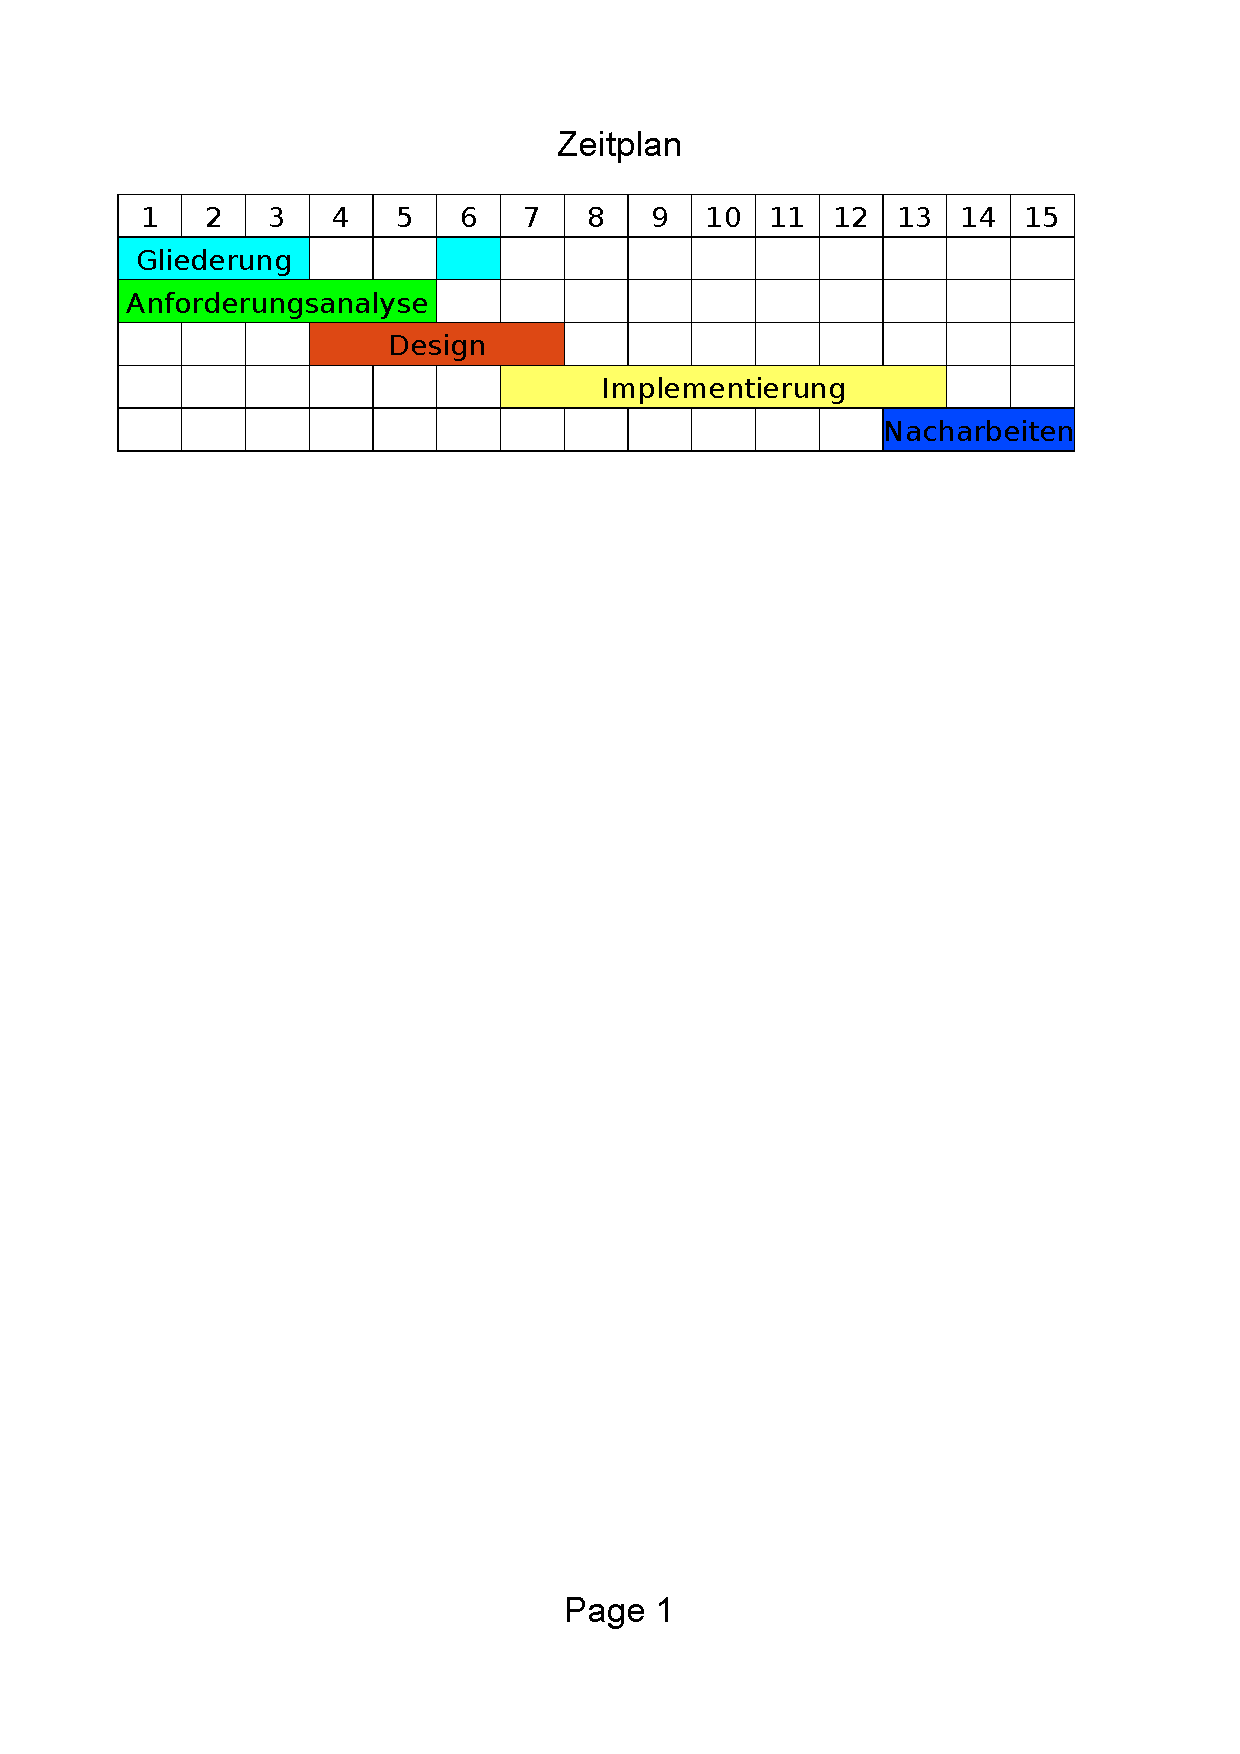
\includegraphics[trim=2cm 22cm 2.5cm 3cm, clip=true, totalheight=0.18\textheight]{zeitplan.pdf}
%\listoffigures
%\listoftables
%\lstlistoflistings
%\listofalgorithms

%\newpage

%\begin{btSect}{es}
% \section{Literaturverzeichnis}
% \label{sec:literaturverzeichnis}
% \btPrintCited
%\end{btSect}

\end{document}
